% !Mode:: "TeX:UTF-8"

\chapter[目标检测算法设计]{目标检测算法设计}[Harbin Institute of Technology Postgraduate Dissertation Writing Specifications]



\section{引言}[Content specification]

目标检测是目标追踪的前提,对于目标检测来说,我们要求它运行速度快,目标召回率与正确率高。
尽管基于深度学习端到端的方案是目前实现成本最低的方案,但是由于计算设备TX2的GPU性能性能较弱,全图推理时间较长(实际测试约为50fps),遂放弃。
\par
本章创新性地提出了一种将传统数字图像处理算法和深度学习相结合的目标检测算法。
通过分析待检测目标的特征不难发现,装甲板是具有非常明显的视觉特征的,两侧有发光灯条,中间有数字图案。通过检测与匹配发光灯条我们可以定位装甲板,
通过数字分类我们可以实现对与装甲板的分类。因此选择将传统数字图像处理与深度学习等技术结合实现装甲板目标的检测。传统数字图像处理算法着重于提高检测算法的召回率,
宁可误选,不可错筛。通过卷积神经网络实现数字分类器,排除掉错误装甲板同时实现装甲板分类。




\section{检测算法的数字图像处理算法设计}

\subsection{灯条提取}
传统视觉算法负责的内容是提取出可能存在装甲板的区域。总体流程是:二值化图像、提取轮廓、灯条判别、灯条匹配装甲板。
因为装甲板左右两侧的灯条的亮度是远高于背景环境的,所以我们可以通过图像二值化方法提取将装甲板的灯条,但是在测试中发现由于装甲板所处的光照环境不同,
对于二值化阈值的选取有着一定的难度,为了让二值化提取能够更好的适应不同的环境我尝试了以下几种方法:\par
1. 使用全局自适应二值化。\par
2. 使用红蓝通道相减的方法对相减之后的图像进行二值化。\par
3. 使用红/蓝通道进行二值化,同时将原图的灰度图二值化,最后将两张图按位与,得到所需的二值化图片。\par

针对以上三种二值化方案我分别进行了测试,首先第一种全局自适应二值化可以很方便的使用OpenCV内置的API实现,不过通过对大量场景下的测试发现由于部分情况下灯条可能与环境中某一处的灯光所重合,
由于二者亮度相差不大,所以自适应二值化会将二者一同处理,造成最终得到的灯条轮廓不闭合,对之后的轮廓筛选造成影响,该方法不具有泛化性,且在复杂光照环境下表现效果一般。\par

第二种方法是基于OpenCV在图像处理中的特点而实现,OpenCV中如果两张图片相减后得到的像素点的值是小于0的那么会直接让它等于0,
而所需要识别的装甲板的灯条只有红蓝两种形式,若将红蓝两通道相减则可以很好的将灯条信息提取出来,但是由于相机参数的影响,
有时会使得灯条的中部为白色,这样的话对应位置红蓝两通道的值相差便不大,
相减之后得到的值几乎为0,二值化之后得到的灯条图像就不再是一个类似矩形的形状,而是一个圆环状,造成轮廓不闭合,
导致之后的轮廓提取出现问题。如图\ref{轮廓不闭合情形}所示。\par
\begin{figure}[H]
    \centering
    
\includegraphics[width=.8\textwidth]{color_channel_subtract.png} 
    \caption{轮廓不闭合情形} 
    \label{轮廓不闭合情形}
\end{figure}


第三种方案通过众多的测试发现在多种情况下都能比较不错的实现对于灯条的提取,
通过分析可以发现由于使用的是灰度图像所以对于场地颜色还有亮度的适应性更强,结合对于颜色通道的二值化图像可以较好的得到最终所需的二值化图像。\par

如果使用OpenCV内置的函数,需要执行两次访存,然后理论上只需要一次访存。因此,在图像二值化这个过程,我并没有使用OpenCV提供的API,而是自己手工实现该功能的。
% \begin{lstlisting}
% void thresh_img(cv::Mat &src, cv::Mat &out, 
%                         int color, int gray_thresh, int color_channel_thresh)
% {
%     cv::Mat grey(src.rows, src.cols, CV_8UC1, cv::Scalar(0));
%     for (int y = 0; y < src.rows; y++)
%     {
%         uchar *cp = src.ptr<uchar>(y);
%         uchar *gp = grey.ptr<uchar>(y);
%         for (int x = 0; x < src.cols; x++)
%         {
%             *gp = (15 * cp[0] + 75 * cp[1] + 38 * cp[2]) >> 7;
%             if (*gp > gray_thresh) 
%             {
%                 if (color == COLOR_BLUE) // Mat默认BGR
%                 {
%                     if (cp[0] > color_channel_thresh)
%                     {
%                         *gp = 255;
%                     }
%                     else 
%                     {
%                         *gp = 0;
%                     }
%                 } 
%                 else 
%                 {
%                     if (cp[2] > color_channel_thresh)
%                     {
%                         *gp = 255;
%                     }
%                     else {
%                         *gp = 0;
%                     }
%                 } 
%             }
%             else
%             {
%                 *gp = 0;
%             }
%             cp += 3;
%             gp++;
%         } 
%     }
%     out = grey;
% }
% \end{lstlisting}

\subsection{装甲板匹配}

经过了二值化之后所有亮度高于灯条或者与灯条亮度一致的区域都会被保留下来
,通过findContours函数寻找图像中所有的轮廓,然后通过OpenCV中拟合矩形的两种的方式(minAreaRect、fitEllipse)获取所有轮廓的外接矩形。
图像上的灯条轮廓是一个不规则的形状,当我们需要描述它的几何信息时无法直接描述,所以我们用灯条的外接矩形来近似代表灯条轮廓。
minAreaRect和fitEllipse都是OpenCV内置的API。minAreaRect方法对于灯条的几何形状信息描述的十分准确;fitEllipse方法对于灯条的角度信息描述的十分准确。
在获取外接矩形后便拥有了它们的长宽以及角度信息,这样便可以利用轮廓的长宽比以及它们的角度进行一个初步的筛选,将满足条件的装甲板存储起来进行下一步的判断。\par


在得到了所有的可能的灯条后需要将灯条两两匹配,同属于一块装甲板的两个灯条。装甲板为一个很标准的矩形,但是由于观测角度、相机成像等因素,观测到的组成装甲板的两个灯条角度差、长度比等信息会有所不同,
但是都还是处于一定范围之内的。通过判断两根灯条的x、y方向上的距离、长宽比、倾斜角度、角度差
等是否满足一定条件可以得到该对灯条是否有可能组成一块装甲板,如果组成一块装甲板的条件通过,则将这一对灯条构成的四边形区域抠出来放入后续的分类器进一步判断。\par
如下图\ref{传统图像处理算法提取多ROI}所示,传统图像处理算法提取出多个可能存在装甲板的ROI。

\begin{figure}[H]
    \centering
    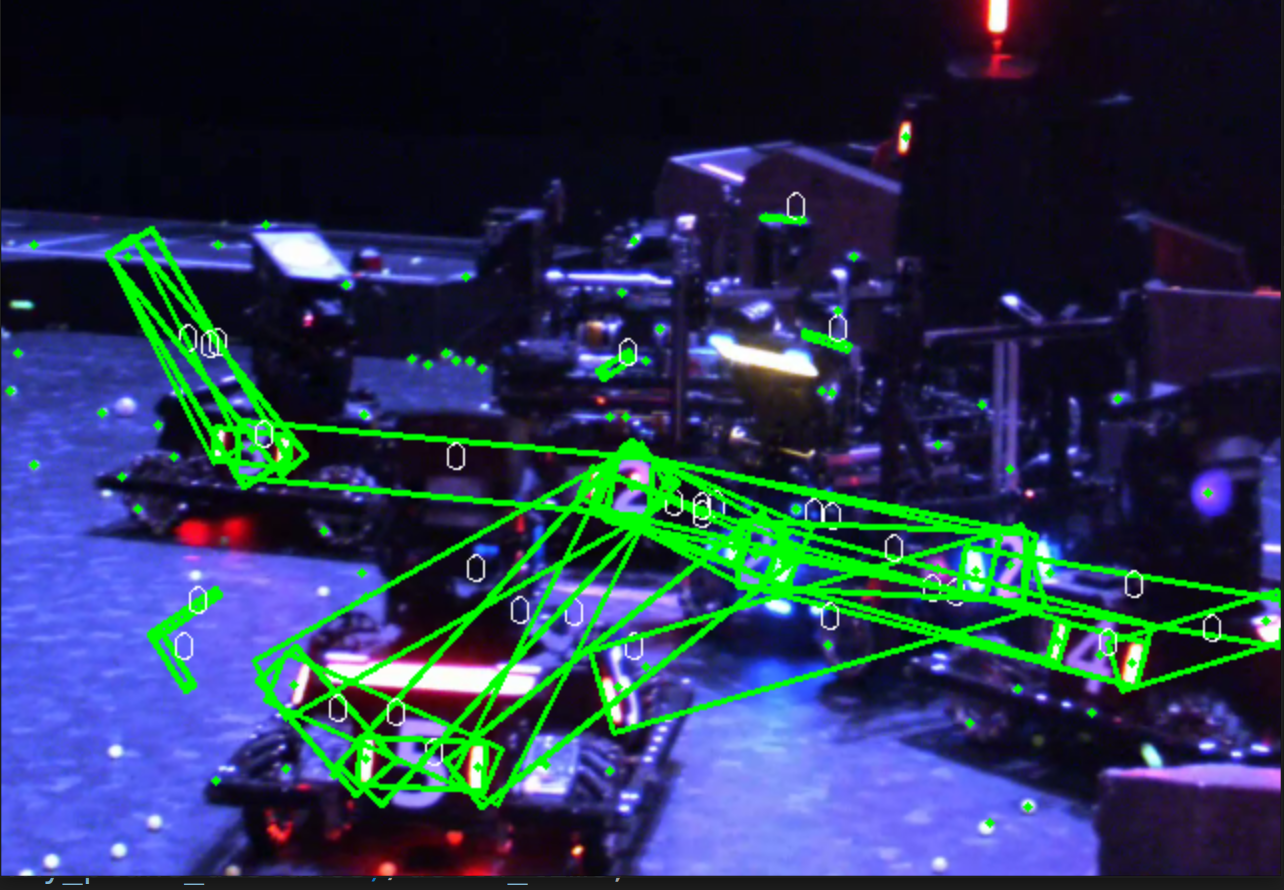
\includegraphics[width=.8\textwidth]{detection_first_stage.png} 
    \caption{传统图像处理算法提取多ROI} 
    \label{传统图像处理算法提取多ROI}
\end{figure}





\section{检测算法的深度学习算法设计}
\subsection{大津二值化算法突显数字特征}
为了尽可能的提高算法运行帧率,则必须尽可能的降低曝光时间,比如,如果算法想要达到300fps,
则最大曝光时间不能超过3.4ms,
又因为装甲板中间的数字图案为不发光体,
所以经常会出现因为图像亮度过低造成数字分类器分类失败的情况。
通过分析装甲板的特征,发现数字图案是白色的,
周围背景是黑色的,尽管数字不发光,但是与背景还是可以区分的,
如果将这一小块区域提取出来使用大津二值化算法\cite{1979A}则能够很好的将背景与图案分割。
如下图\ref{ostu}所示,左图为原图,右图为经过大津二值化算法处理过后的图。
\begin{figure}[H]
    \centering
    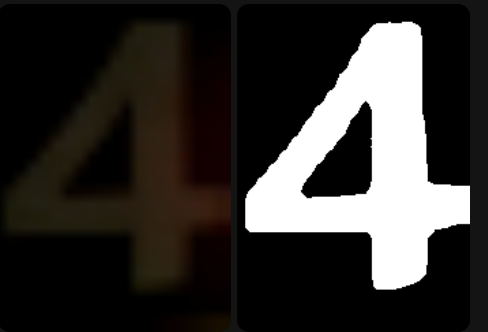
\includegraphics[width=.8\textwidth]{ostu.png} 
    \caption{大津二值化算法效果图,左图为原图,右图为二值化之后的图像} 
    \label{ostu}
\end{figure}




\subsection{卷积神经网络实现图像分类}

为了防止出现误识别的情况,提取到“装甲板”对应的ROI区域后需要将它们放入分类器去进行分类,此外对于不同的兵种(装甲板对应不同的数字)击打的优先级是不同的,因此对于装甲板类别的判断是非常重要的。\par
目前对于图像分类的方式有许多种,比如基于卷积神经网络方案(如ResNet\cite{2016Deep})和传统机器学习(如SVM)
等。我们的任务是实现装甲板分类,装甲板的特征比较简单但是类别较多,同时还需要具备对于负样本的判断能力,
基于这几个特点选用卷积神经网络实现图像分类任务。
\begin{figure}[H]
    \centering
    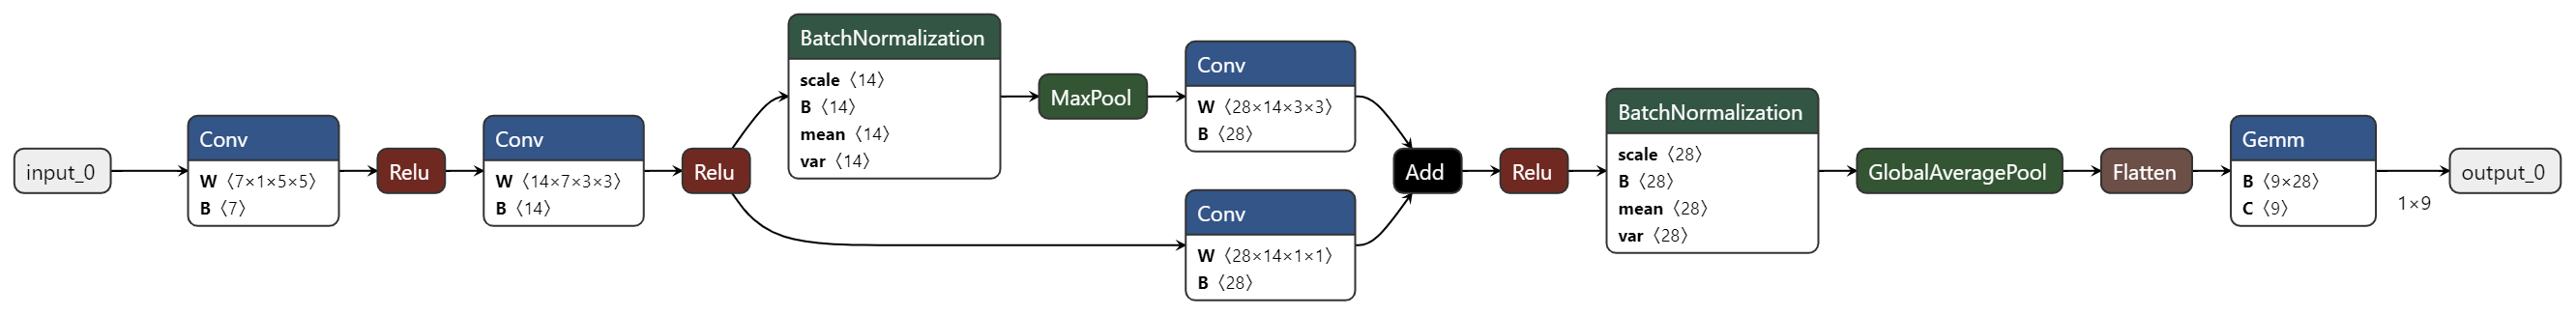
\includegraphics[width=.8\textwidth]{classify_network_structure.png} 
    \caption{分类器网络结构} 
    \label{分类器网络结构}
\end{figure}
全连接的神经网络虽然形式简单同时也能获得一个较高的准确度,
但是全连接层巨大的参数量会对运行时间造成很大的影响,因此我们考虑使用全局平均池化去解决参数量大的问题,
可使用全局平均池化虽然减少了参数量却丢失了许多信息,测试发现模型收敛后无法达到一个较高的准确度。
对于此问题所采用的解决方案是在两层卷积层之后引入一个残差块,将前两层卷积所提取到的特征信息与第三层卷积层的计算结果融合起来,
然后再去使用全局平均池化,经过测试发现最终它所能达到的准确超过全连接神经网络。网络结构如图\ref{分类器网络结构}所示。


下图\ref{网络训练时准确率与LOSS值收敛过程}展示训练时的准确率、LOSS值的变化。
\begin{figure}[H]
    \centering
    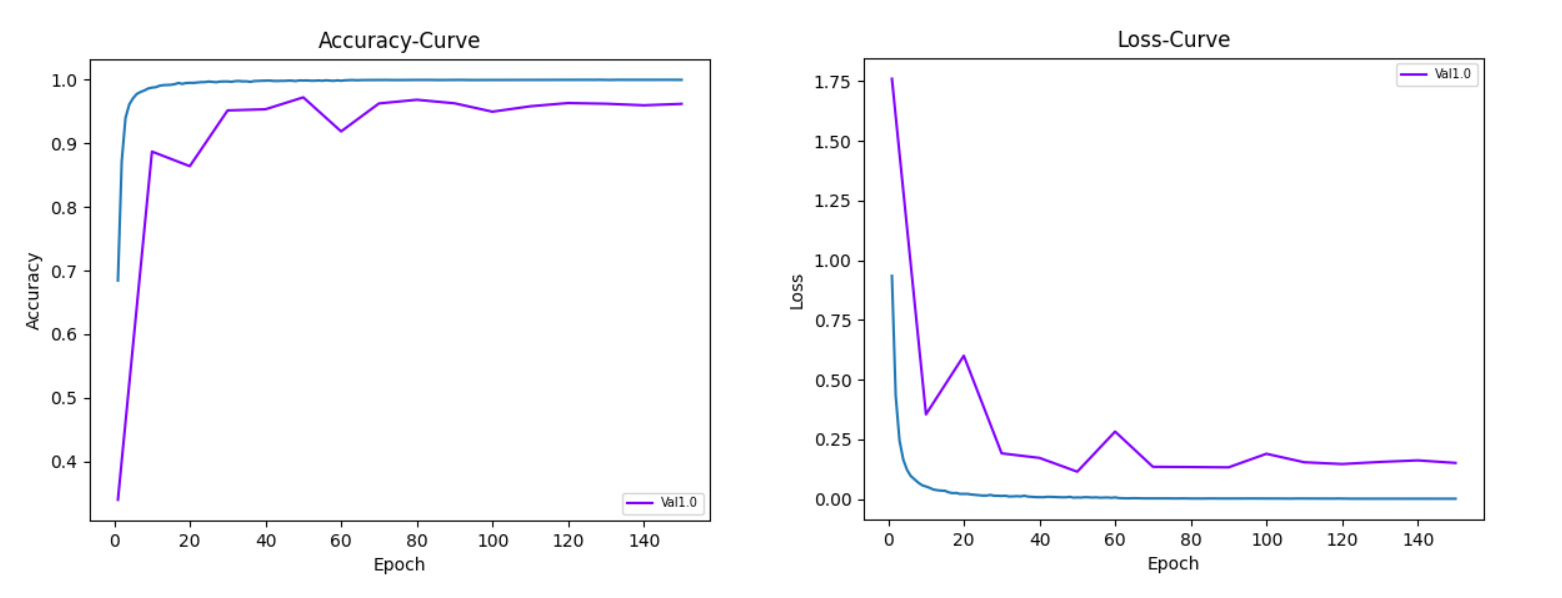
\includegraphics[width=.8\textwidth]{train.png} 
    \caption{网络训练时准确率与LOSS值收敛过程} 
    \label{网络训练时准确率与LOSS值收敛过程}
\end{figure}


下图\ref{分类器测试结果}展示训练后的神经网络在面对新数据时的表现。可以看到神经网络分类器对于模糊、有噪声干扰、形状不一的图片都有很好的表现。
\begin{figure}[H]
    \centering
    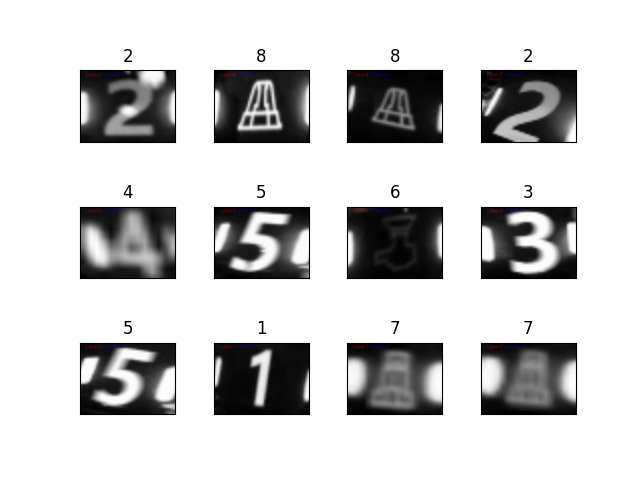
\includegraphics[width=.8\textwidth]{classify_demo.png} 
    \caption{分类器测试结果} 
    \label{分类器测试结果}
\end{figure}

下图\ref{识别算法最终效果展示}展示经过神经网络分类器判别之后得到的装甲板。可以看到经过神经分类器后,一些误识别的区域排除,只留下存在装甲板的区域。
\begin{figure}[H]
    \centering
    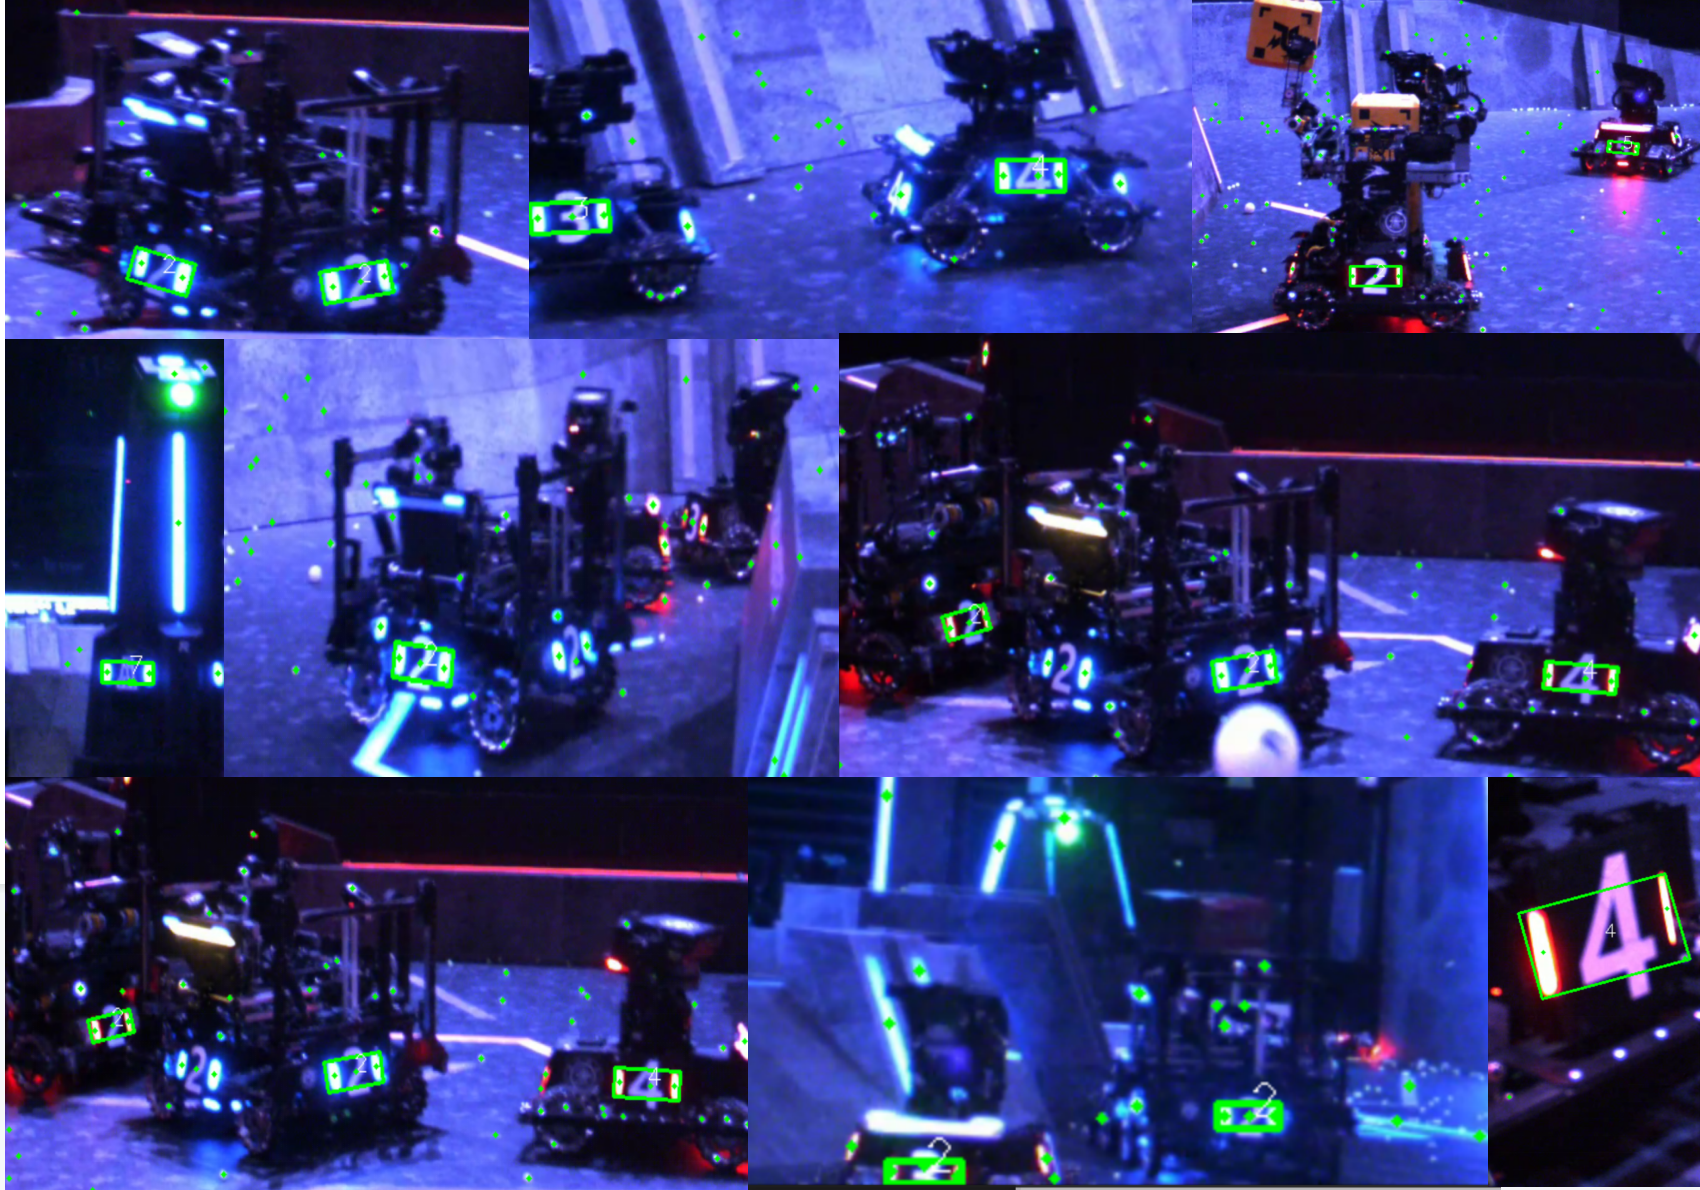
\includegraphics[width=.8\textwidth]{detection_final_result.png} 
    \caption{识别算法最终效果展示,识别到的装甲板被绿色框框出} 
    \label{识别算法最终效果展示}
\end{figure}

\section{本章小结}
将传统数字图像处理与深度学习等技术结合实现装甲板目标的检测。将算法部署在NVIDIA TX2 上,运行平均帧率150fps+,召回率98\%,正确率99\%。检测算法性能满足系统要求。



